\documentclass[border=3pt]{standalone}
\usepackage{tikz}
\usetikzlibrary{patterns}
\begin{document}
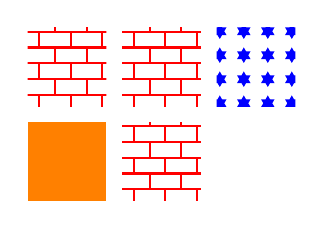
\begin{tikzpicture}
  \fill[white] (0,0) rectangle (3.4,2.2);
  \begin{scope}[pattern=bricks,pattern color=red]
    \pattern (0,1.2) rectangle (1,2.2);
    \path[pattern] (1.2,1.2) rectangle (2.2,2.2);
    \pattern[pattern=sixpointed stars,pattern color=blue] (2.4,1.2) rectangle (3.4,2.2);
  \end{scope}
  \begin{scope}[fill=orange]
    \pattern (0,0) rectangle (1,1);
  \end{scope}
  \path[pattern=bricks,pattern=none,pattern,pattern color=red] (1.2,0) rectangle (2.2,1);
  \pattern[pattern=none] (2.4,0) rectangle (3.4,1);
\end{tikzpicture}
\end{document}
